\subsection{Réserves de Liquidités}

\begin{frame}
    \frametitle{Présentation du concept de réserve de liquidité}
    \begin{itemize}
        \item Smart Contract fournissant une solution d'échange d'actifs
        \begin{itemize}
            \item Des "holders" déposent des actifs dans la pools.
            \item Des "traders" échangent des actifs contre des tokens de la pools.
        \end{itemize}
    \end{itemize}    
    \begin{figure}
        \centering
        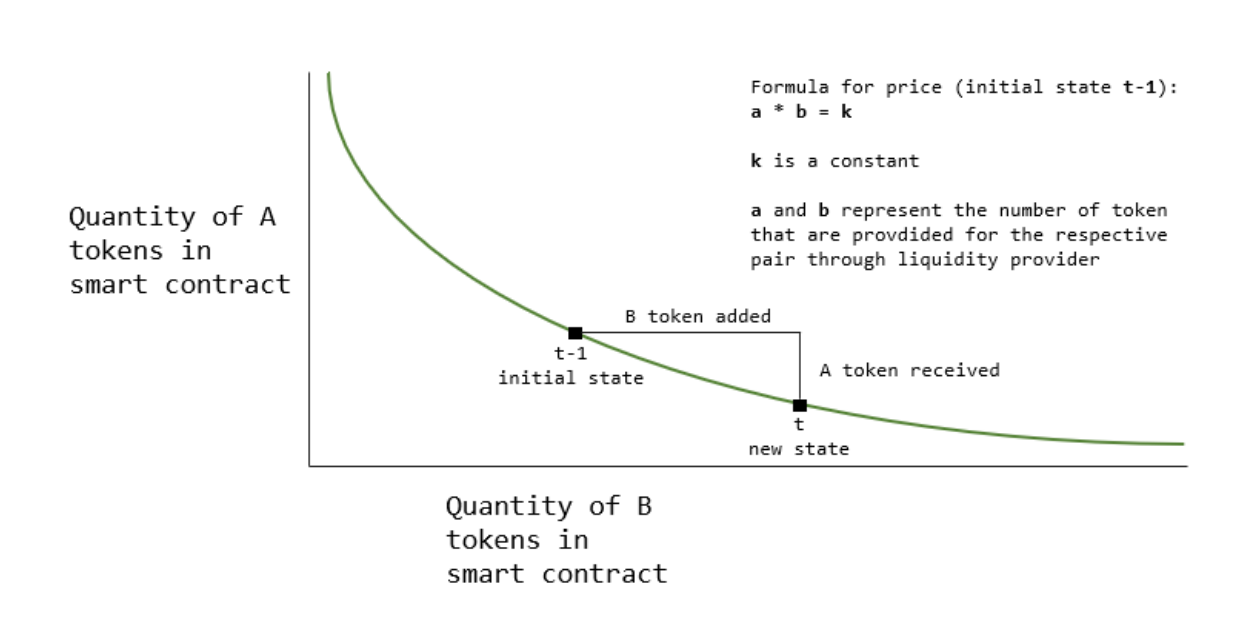
\includegraphics[scale = 0.22]{decentralisation/reserve_liquidite.png}
    \end{figure}
\end{frame}

% schema:
% @startuml
% hide footbox
% actor Bob as B
% actor Carole as C
% participant  "Reserve de Liquidité" as R
% actor Alice as A

% B -> R : dépose 100 A
% R --> B : gagne 100 LP
% C -> R : dépose 100 B
% R --> C : gagne 100 LP
% ...
% A -> R : Depose 10 A
% R --> A : Retire 9 B
% R --> B : Gagne 0.4 LP
% R --> C : Gagne 0.4 LP
% R --> R : Garde 0.1 LP
% @enduml

\begin{frame}
    \frametitle{Présentation du concept de réserve de liquidité}   
    \begin{figure}
        \centering
        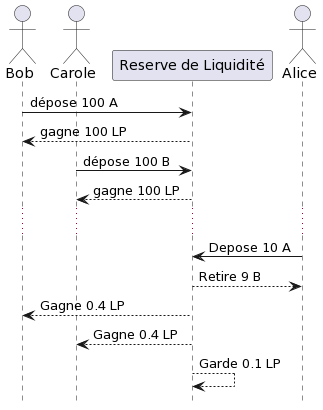
\includegraphics[scale = 0.5]{decentralisation/reserve_liquidite_explain.png}
    \end{figure}
\end{frame}

\subsection{CVE-2021-3006}
\begin{frame}
    \frametitle{CVE-2021-3006}
    \begin{itemize}
        \item Concerne une erreur d'implémentation dans les reserve de liquidités du réseau SEAL.
        \item Details du fonctionnement de SEAL:
        \begin{itemize}
            \item Les "holders" gagnent une comission à chaque transaction sous forme de jetons LP.
            \item Ils peuvent ensuite retirer leurs jetons LP contre des actifs grace à l'appel de la fonction \textit{breed()}.
            \item Cette fonctions à pour effet secondaire d'utiliser $1,6\%$ des récompenses des "holders" pour les reinvestir dans la reserves.
        \end{itemize}
    \end{itemize}   
\end{frame}

\begin{frame}
    \frametitle{CVE-2021-3006}
    \begin{figure}
        \centering
        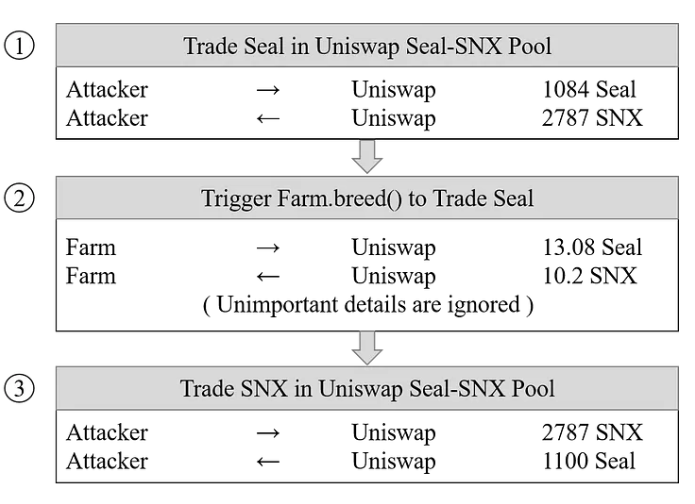
\includegraphics[scale = 0.3]{decentralisation/cve_2022_3006.png}
    \end{figure}
\end{frame}

\begin{frame}
    \frametitle{CVE-2021-3006}
    \begin{figure}
        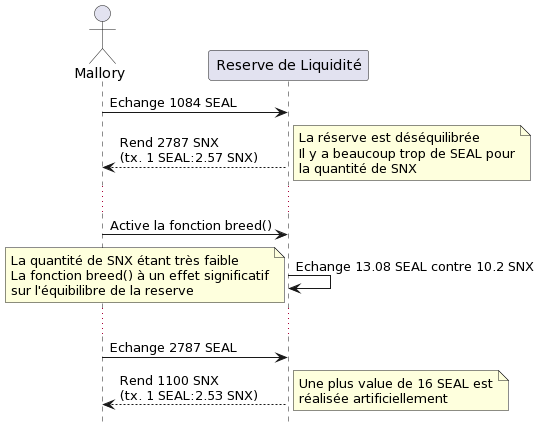
\includegraphics[scale = 0.5]{decentralisation/cve_2021_3006_explain.png}
        \centering
    \end{figure}
\end{frame}